\svnidlong
{$HeadURL$}
{$LastChangedDate$}
{$LastChangedRevision$}
{$LastChangedBy$}
\framebox{Author: \svnauthor|Rev: \svnrev|Last change: \svndate}% - URL: \url{\svnkw{HeadURL}}}
\section{Results}
Results of the aforementioned steps are shown in figure~\ref{fig:wide field scan}. Figure~\ref{subfig:wfs-sub} shows exemplary projection images from overlapping subscans prior to correction and normalization. Figure~\ref{subfig:wfs-mrg} shows a merged projection image prior to reconstruction and figure~\ref{subfig:wfs-slice} shows the end-result of such a wide field scan, a reconstructed slice of the whole sample with a FOV of \unit{5.734}{\milli\meter} --- approximately three times the size of what can be achieved with one single scan.

\begin{figure}[p] % [tb] for small, [p] for big pictures
	\centering
	%\begin{minipage}{0.618\textwidth}
	\centering
	\renewcommand{\imsize}{0.25\textwidth}
	\subfloat[Flat field image]{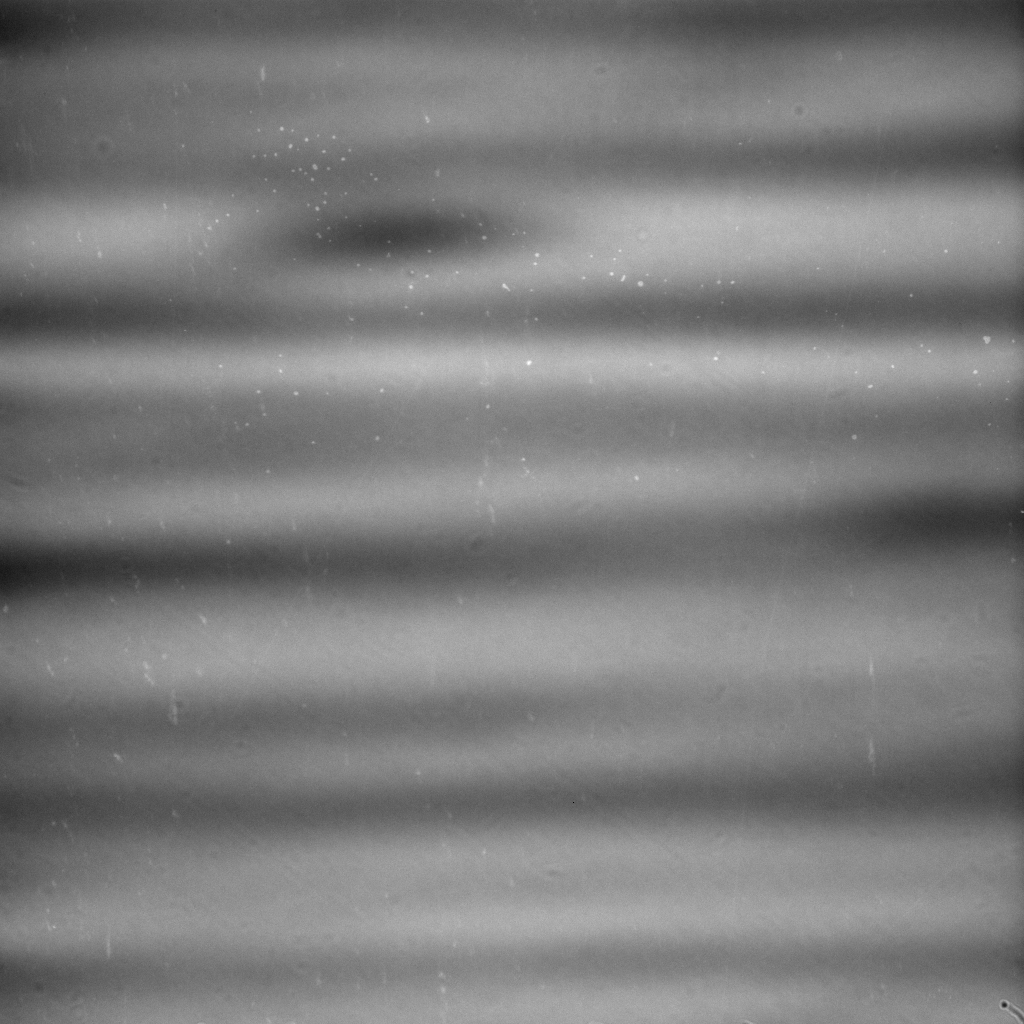
\includegraphics[width=\imsize]{img/correctedprojections/R108C10B_s10012}\label{subfig:flat}}\subfloat[Uncorrected projection images from three overlapping subscans. Each image has an original size of \numprint{1024}$\times$\numprint{1024} pixels and covers a FOV of approximately \unit{0.7}{\milli\meter}. The scans shown above overlap each other by approximately 100 pixels.]{\label{subfig:wfs-sub}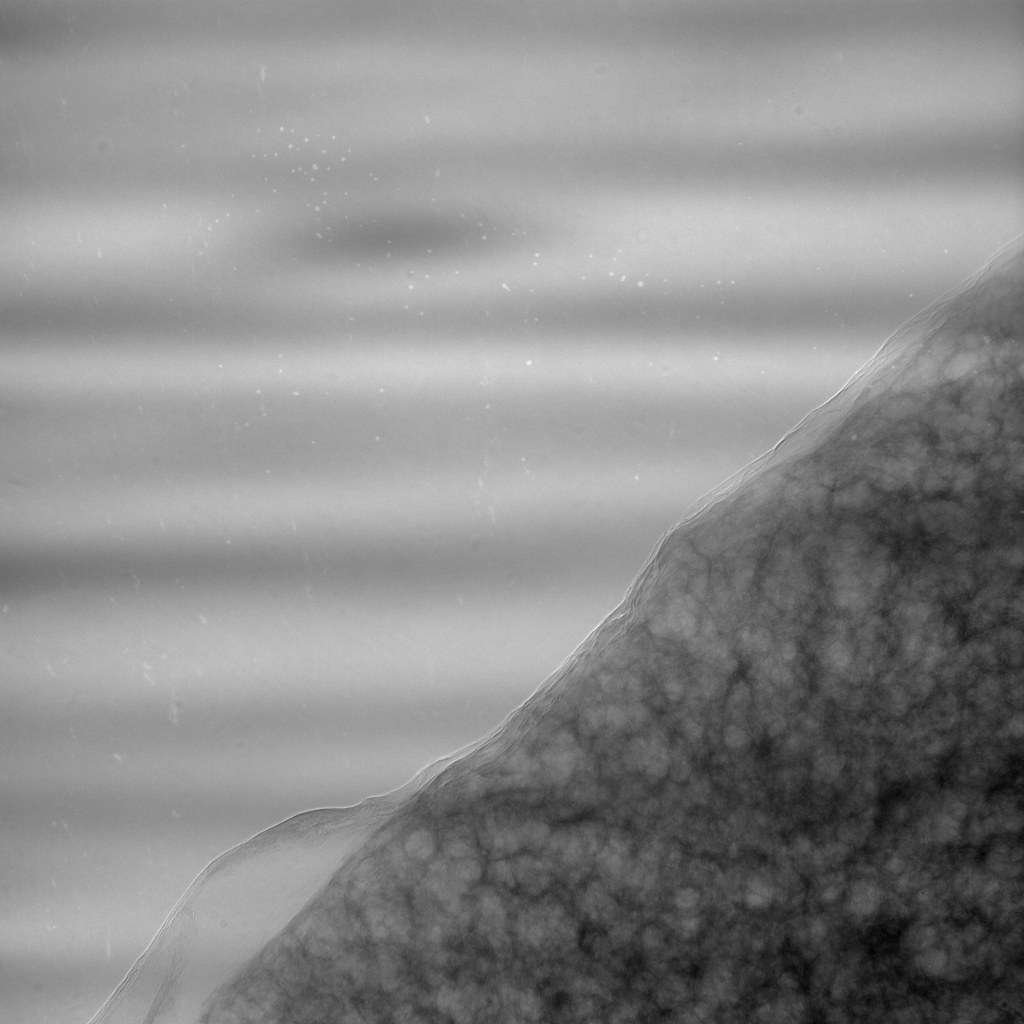
\includegraphics[width=\imsize]{img/correctedprojections/R108C10B_s10013}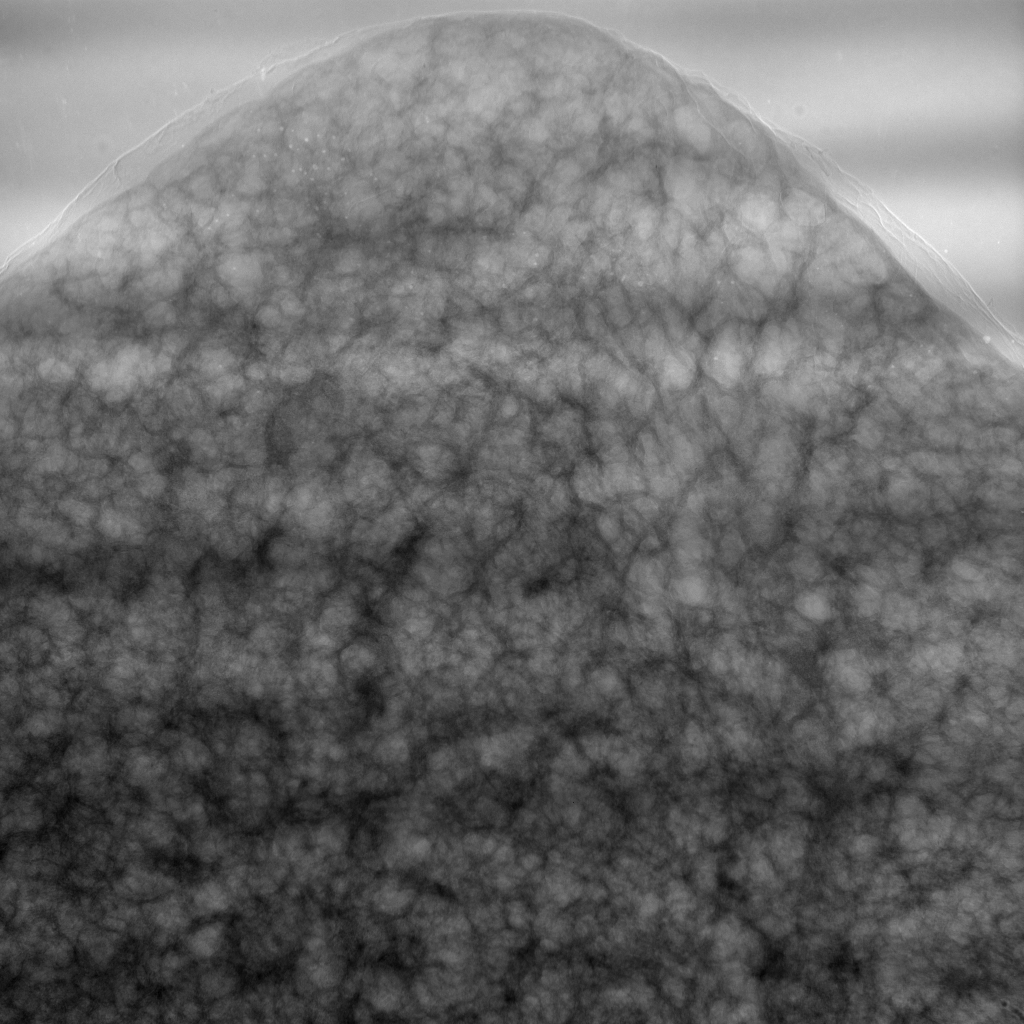
\includegraphics[width=\imsize]{img/correctedprojections/R108C10B_s20013}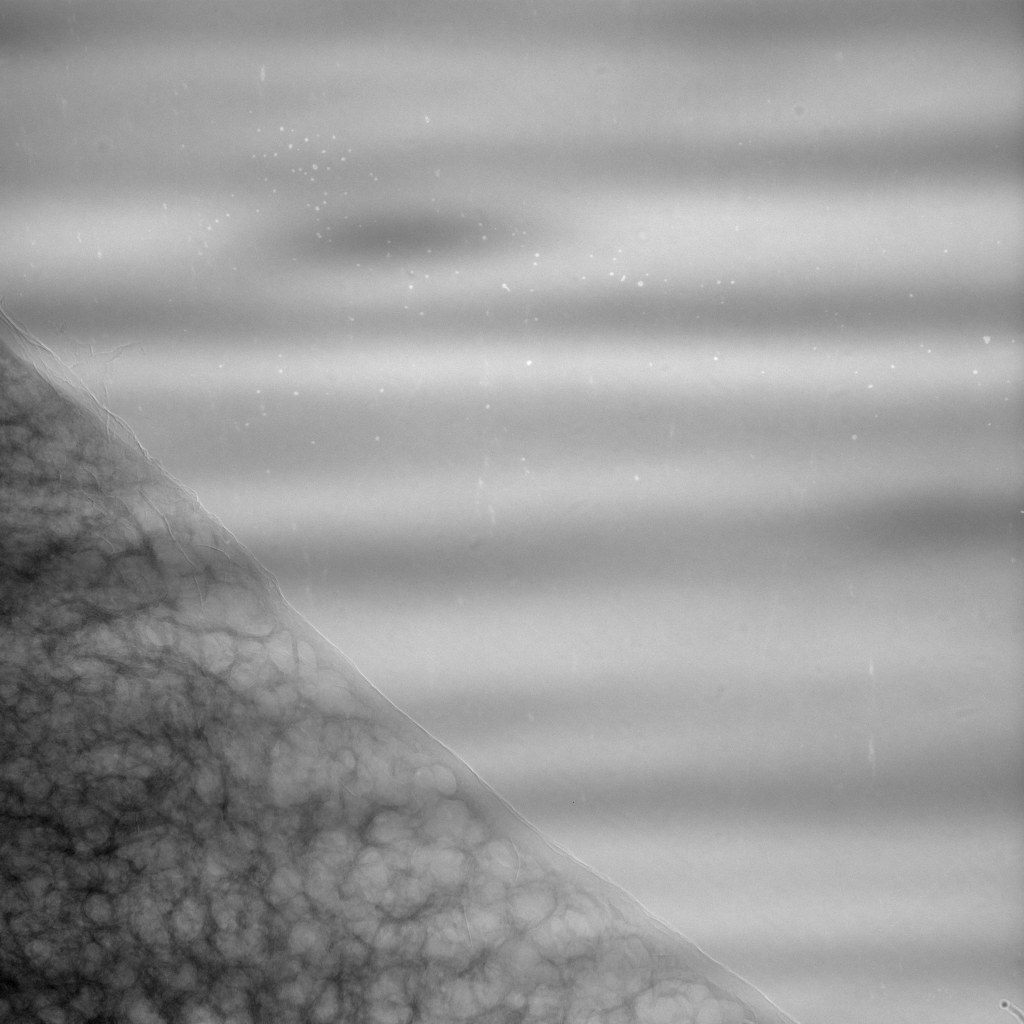
\includegraphics[width=\imsize]{img/correctedprojections/R108C10B_s30013}}
	\renewcommand{\imsize}{\textwidth}
	\subfloat[Merged and corrected projection composed from the three subscans shown in \subref{subfig:wfs-sub}. The images have been corrected with the flat image shown in~\ref{subfig:flat}, the correct cutting line has been calculated, and the images have been merged into one big projection image. This merged projection has a size of \numprint{2994}$\times$\numprint{1024} pixels. This particular sample consists of \numprint{4678} such projection images (see section~\ref{subsec:image processing} for details). A slice reconstructed from a set of merged projections like this one is shown in \subref{subfig:wfs-slice}.]{
	\label{subfig:mrg}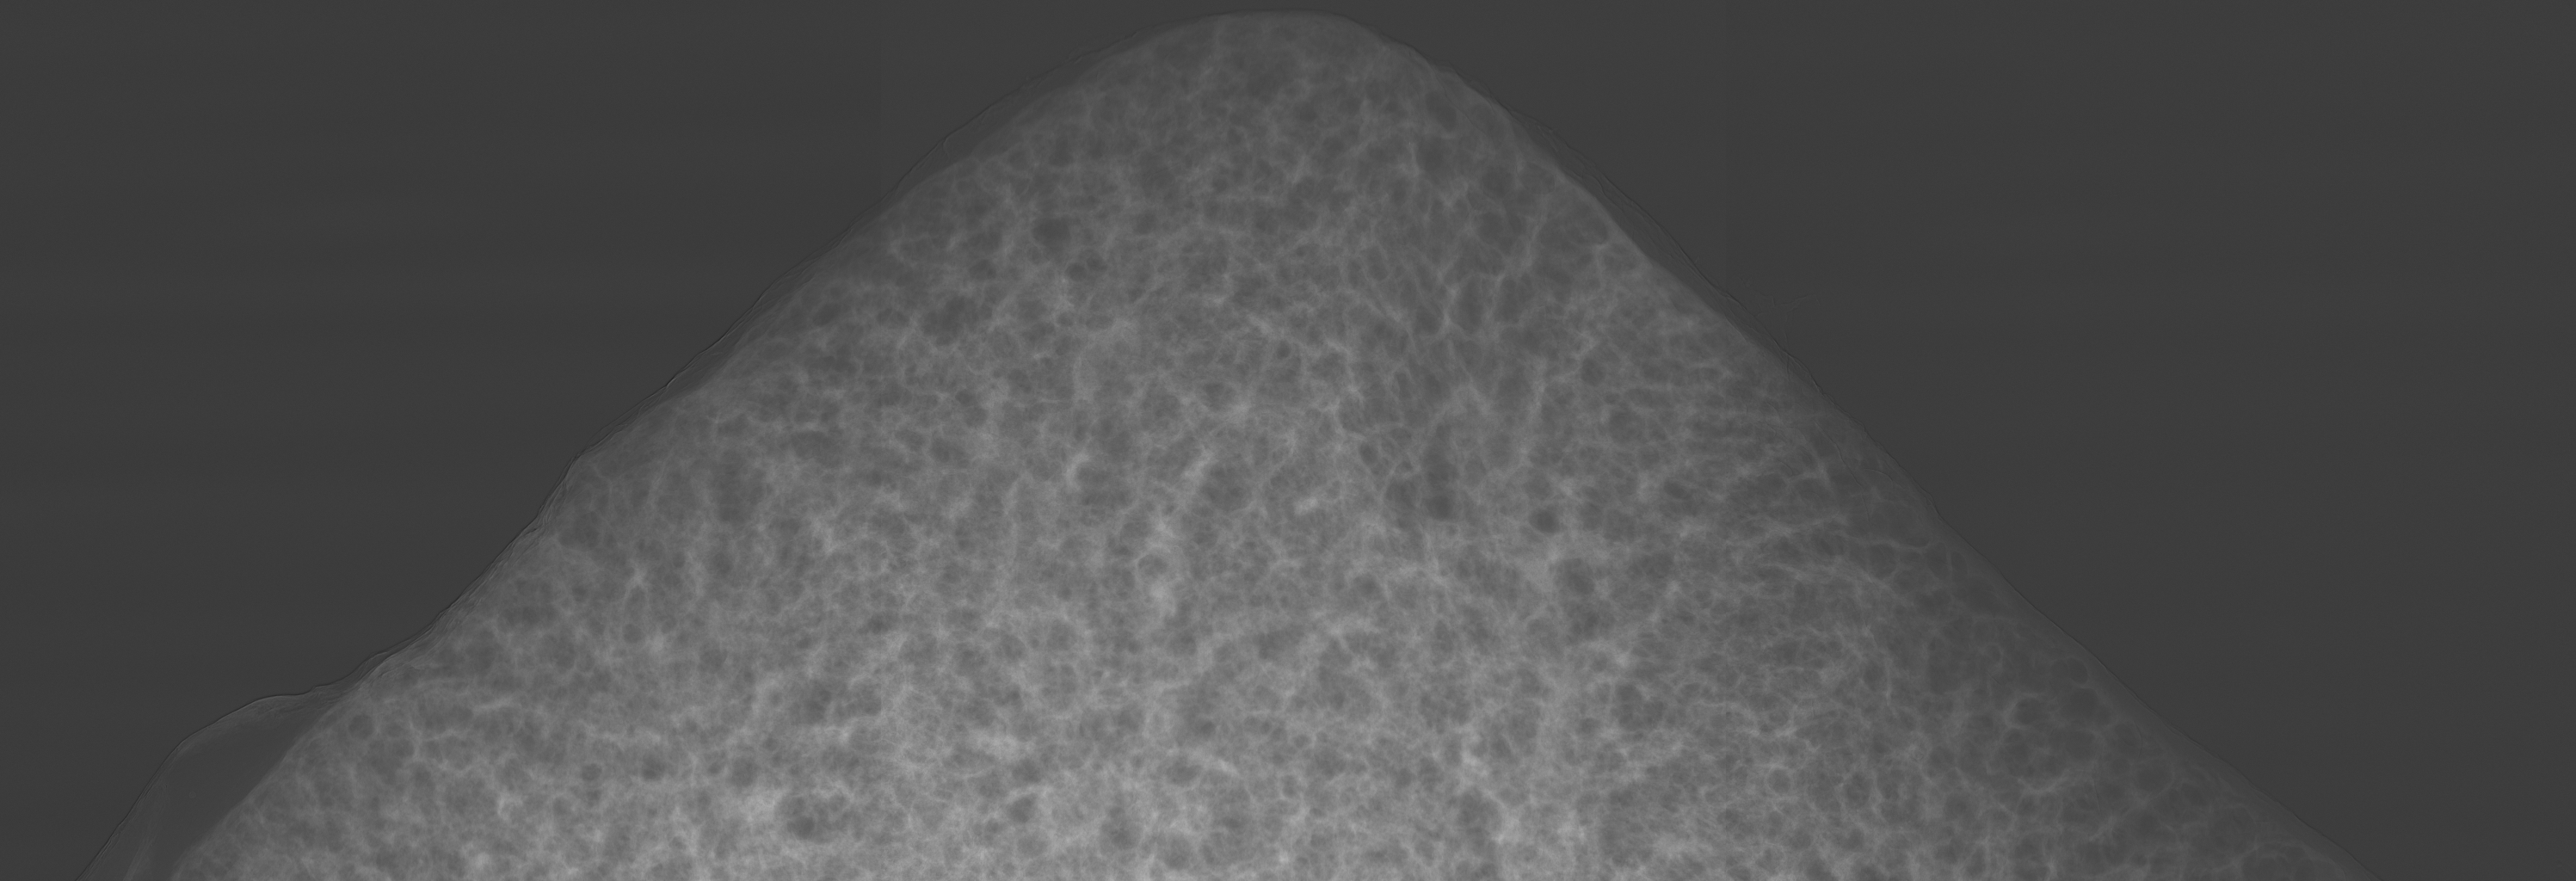
\includegraphics[width=\imsize]{img/correctedprojections/R108C10B_merge0001}
	}
	\\
	\subfloat[Detailed view of a reconstructed slice of the full data set with a an original size of \numprint{2994}$\times$\numprint{2994} pixels, covering a FOV of approximately \unit{2.5}{\milli\meter}. This cropped slice has a size of \numprint{2665}$\times$\numprint{1087} pixels ]{\label{subfig:wfs-slice}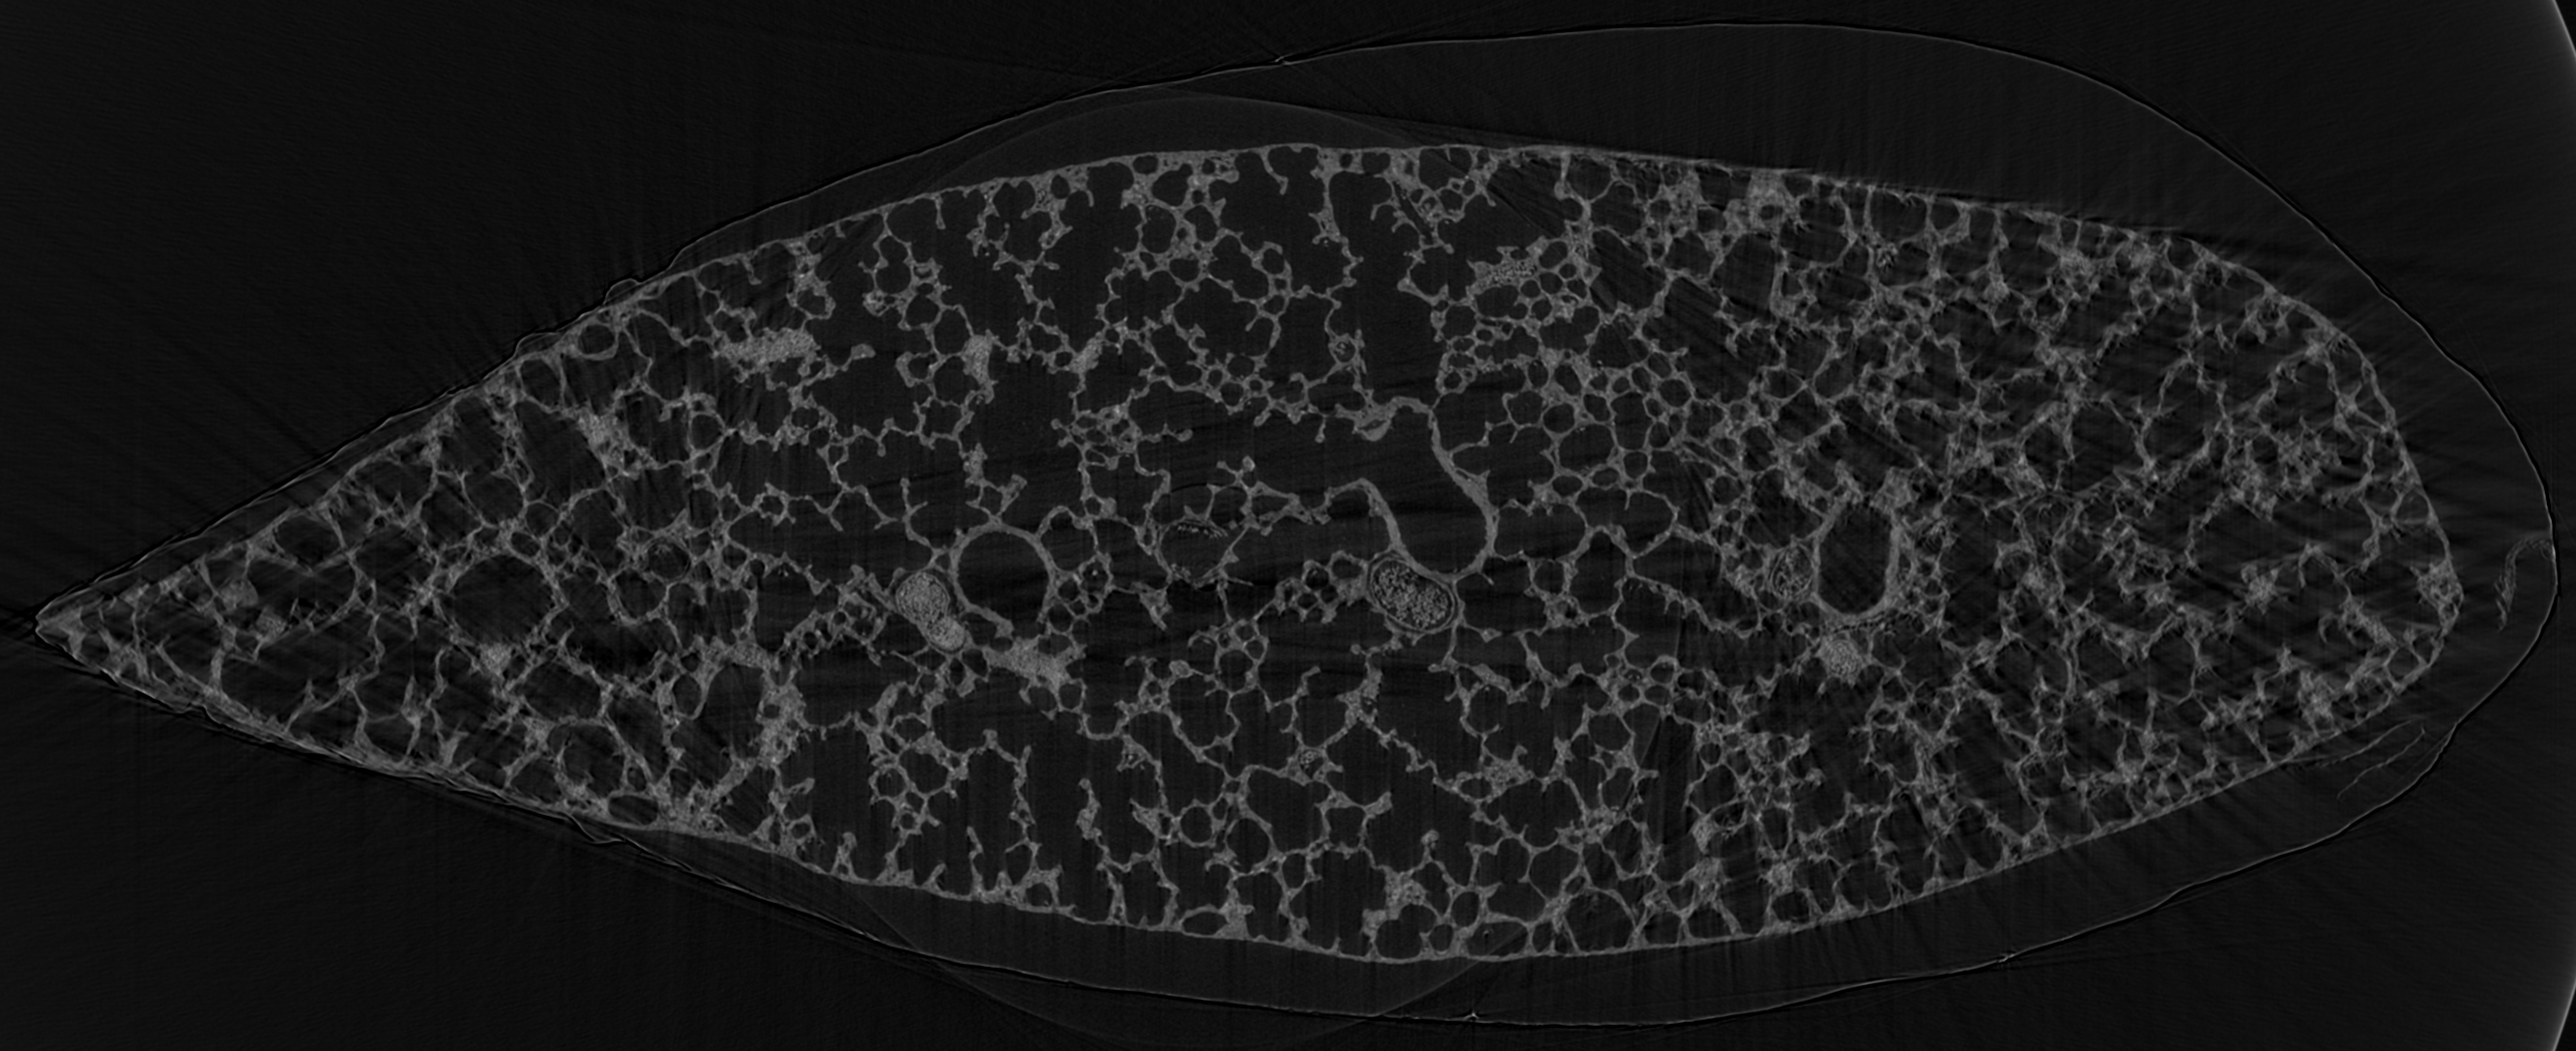
\includegraphics[width=\imsize]{img/correctedprojections/R108C10B_merge0989_rec_8bit_crop}}
	\caption{Different stages of a wide field scan of a sample obtained from a Sprague-Dawley rat 10 days after birth, scanned at a beam energy of \unit{12.6}{\kilo\electronvolt}.}
	\label{fig:wide field scan}
	%\end{minipage}
\end{figure}